\textbf{Software Testing }\\
Obwohl unser Projekt relativ klein ist, wollten wir, wo immer möglich, automatisierte Testfälle einbeziehen.

Für das Frontend haben wir End-to-End Testfälle mit Cypress geschrieben.

So können wir in Sekundenschnelle feststellen, ob etwas in unserer Anwendung defekt ist.

Ein mögliches Szenario ist, dass eine Komponente, die in anderen Komponenten verwendet wird, geändert wurde, ohne zu berücksichtigen, dass sie in einer anderen Komponente für einen anderen Zweck verwendet wurde.

Das ist der Fall bei der Komponente AvatarImage.
%---
Dies ist eine Funktionskomponente, die 3 Parameter erhält: Größe des Bildes, Bild-URL und Benutzername.

Zu Beginn des Projekts wurde nicht daran gedacht, die Größe des Bildes über einen Parameter dieser Funktion zu steuern. Im Laufe des Projekts wurde uns klar, dass wir die Logik in diesem Element wiederverwenden konnten.

Innerhalb der Komponente wird geprüft, ob eine URL existiert, und wenn ja, wird das mit dem Link verbundene Bild gezeichnet. Falls es keine URL  angegeben wurde, werden die ersten beiden Buchstaben des Benutzernamens verwendet, um ein Standardsymbol zu erzeugen.

In der aktuellen Version des Codes wird diese Komponente in vier anderen Komponenten wieder verwendet.
Wenn das Projekt weiter wachsen würde, würde auch die Möglichkeit von Fehlern im Code zunehmen. Und es wäre schwieriger, sie zu finden.

Ohne automatisierte Tests müssten Sie normalerweise manuell prüfen, ob die übergeordneten Komponenten noch wie erwartet funktionieren.


%code
\begin{lstlisting}
//in constants.js sind Standard-Testdaten
import * as c from "../constants.js"

const qtyLanguages = 101
const qtyGenders = 8
const qtyInGameRoles = 6

describe("Check if all profile elements have been rendered", () => {
  it("Login with existing account", () => {
    cy.typeLogin(c.email, c.password)
  })

  it("Username was rendered", () => {
    cy.get('#username').should("be.visible")
  })

  it("Gender selection was rendered", () => {
    cy.get('#dropdown-gender').should(
      "be.visible")
  })

it(`Gender options is not empty and >= to ${qtyGenders}`, () => {
  cy.get('#dropdown-gender').click()
  cy.get(`.dropdown-menu > :nth-child(${qtyGenders})`).should(
      "be.visible")
  //close the dropdown
  cy.get('#dropdown-gender').click()

  })

  it("Language selection was rendered", () => {
    cy.get("#avaliableLanguages > .dropdown > #dropdown-languages").should(
      "be.visible")
  })

  it(`Language options is not empty and has at least ${qtyLanguages} options`, () => {
    cy.get("#dropdown-languages").click()
    cy.get(`.dropdown-menu > :nth-child(${qtyLanguages})`).should( "be.visible")
    //close the dropdown
    cy.get("#dropdown-languages").click()
  })

  it("InGameRole selection is there", () => {
    cy.get("#avaliableIngameRoles > .dropdown > #dropdown-ingamerole").should(
      "be.visible")
  })

it(`InGameRole options is not empty and has at least ${qtyInGameRoles} options`, () => {
    cy.get("#dropdown-ingamerole").click()
    cy.get(`#avaliableIngameRoles > .dropdown > .dropdown-menu > :nth-child(${qtyInGameRoles})`).should( "be.visible")
    //close the dropdown
    cy.get("#dropdown-ingamerole").click()
  })

 it("AboutMe was rendered", () => {
    cy.get('#aboutMe').should("be.visible")
  })
  
})

\end{lstlisting}

%%POSIBLEMENTE ESTE NO ES ELMEJOR EJ PUESTO QUE NO SE ESTA PROBANDO EL TAMANIO LAS IMAGENES EN LAS PRUEBAS DE CYPRESS
%% SIN EMBARGO EL HECHO DE REUTILIZAR LOGICA DE CIERTOS ELEMENTOS ES MUY RELEVANTE Y DEBERIA SER INCLUIDA EN OTRA PARTE %DEL REPORTE
%BUSCAR OTRO EJ. DONDE EL TESTING COBRA MAS RELEVANCIA

\subsection{Die Testfälle für unser Projekt}
\paragraph{}
Ansicht der laufenden Testfälle.
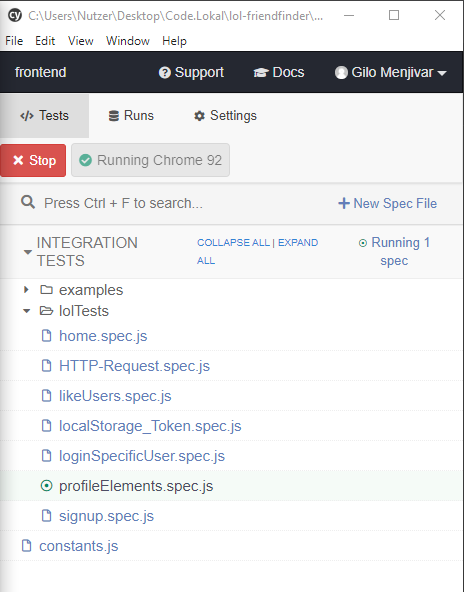
\includegraphics[scale=0.60]{Cy_Test_Cases}
\\
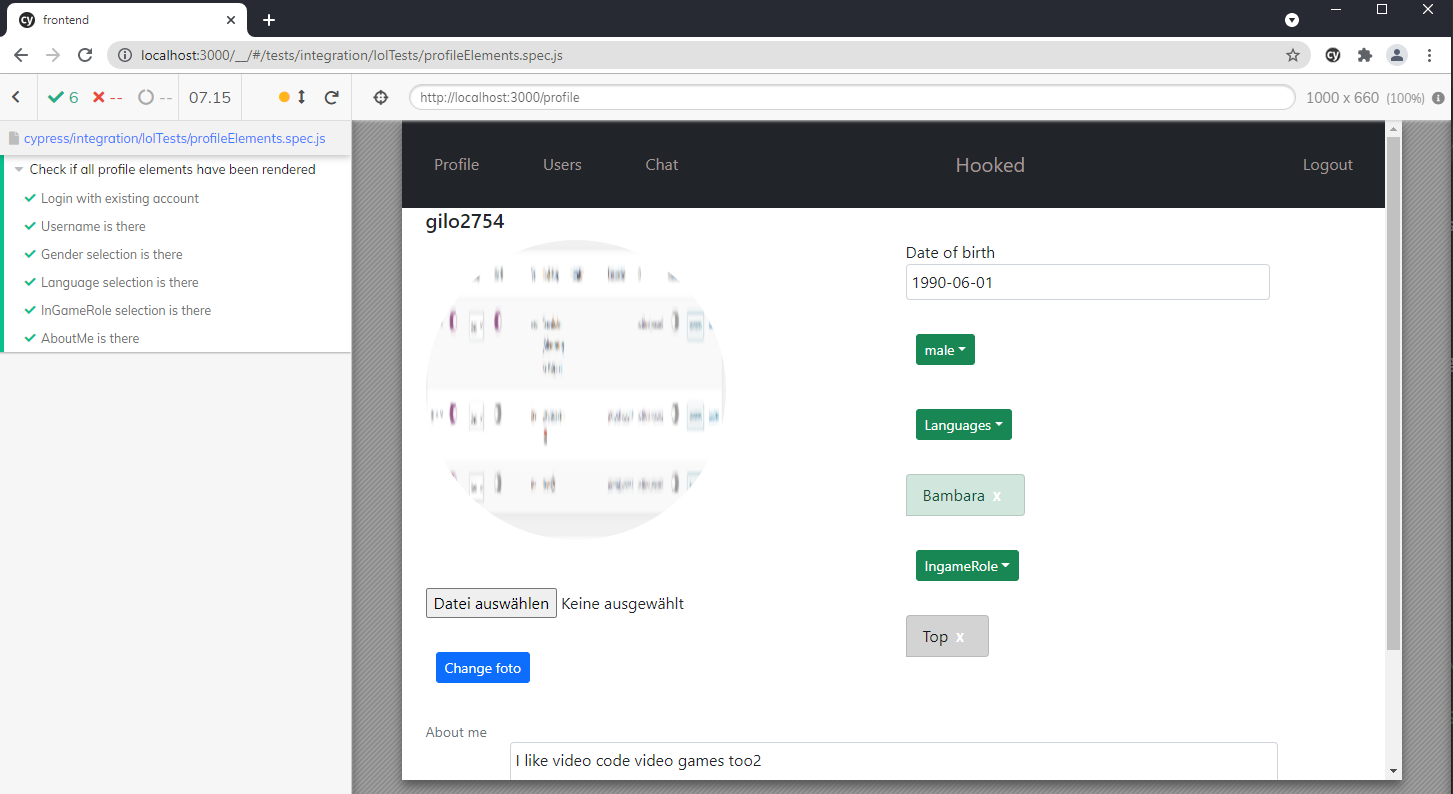
\includegraphics[scale=0.20]{Cy_Test_running}

\newpage
\textbf{home.spec.js}\\
Prüfen Sie, ob die Startseite „Home“ gerendert wurde.
\\\\
\textbf{HTTP-Request.spec.js}\\
\\\\
\textbf{likeUsers.spec.js}\\
Mit diesem Testfall wird überprüft, ob nach der Vergabe von einem „Like“ oder einem „Dislike“ ein anderer Nutzer angezeigt wird.
\\\\
\textbf{Testfall localStorage Token}\\
Hier wird der Wert des JSON-Web-Tokens zu verschiedenen Zeitpunkten überprüft.
Die Erwartung ist, dass das Token null ist, wenn der Benutzer nicht angemeldet ist.
Dieses Token wird in localStorage gespeichert.
Es besteht auch die Möglichkeit, dass das Token abgelaufen ist, wodurch alle Anfragen an den Server, die eine Authentifizierung erfordern, unmöglich werden.
\\\\
\textbf{profileElements.spec.js}\\
Der Testfall prüft, ob die Elemente und Komponenten der Komponente Profil gerendert wurden und sichtbar sind. Diese Elemente sind userName, Gender und AboutMe. Die Komponenten sind Language und InGameRole.

Außerdem wird überprüft, ob Komponenten, ein Element „Dropdown“ enthalten, eine Mindestanzahl von Elementen enthalten, die angezeigt werden müssen. 
\\
\textbf{signUp.spec.js}\\
Dieser Testfall erstellt einen neuen Benutzer mit einer zufälligen E-Mail und einem zufälligen Benutzernamen.  \\
\\
\textbf{Commands bei Cypress}\\
In den Testfällen gibt es Aktionen, die sich immer wieder wiederholen, zum Beispiel die Anmeldung eines Nutzers.
Zu diesem Zweck wurde in Cypress ein wiederverwendbarer Befehl definiert.
\begin{lstlisting}
    Cypress.Commands.add("typeLogin", (email, password) => {
        cy.visit("/login")
    
        cy.get("[id=email-input]").type(email).should("have.value", email)
    
        cy.get("[id=password-input]").type(password).should("have.value", password)
    
        cy.get("[id=btn-submit]").click()
    })
\end{lstlisting}
Mit anderen Worten, es handelt sich um eine Funktion, die zwei Parameter, E-Mail und Passwort, erhält. 
Beide Parameter werden in die entsprechenden Eingabefelder eingetragen, abschließend wird die Eingabetaste gedrückt.
Diese Funktion kann in jedem anderen Testfall aufgerufen werden, ohne dass sie importiert werden muss.

%Ergebnise der ganzen Testlauf